%! Author = Miriam Streit
%! Date = 17.06.23

\section{Verteilungssicht}
\label{sec:verteilungssicht}
Die Applikationen werden in Docker-Container gebaut, damit sie lauffähig sind. Bei Spring Boot und Micronaut reichen dafür Maven und Java als Abhängigkeit aus. Bei Jakarta EE wird ein Glassfish-Base-Image benötigt.
Das Frontend wird in einem ersten Schritt gebaut und dann mit einem Nginx Image zusammen verpackt, damit es als Container lauffähig ist. Die Datenbank besteht aus einem Postgres-Image.

Die gesamte Applikation soll schlussendlich auf einem Kubernetes-Cluster betrieben werden. Dafür wird in dieser Projektarbeit Minikube verwendet. Dabei befindet sich alles auf der lokalen Maschine.
Die verschiedenen Services werden in Docker Container auf dem Cluster deployed. Pro Service und für die Datenbank wurde ein Deployment benötigt. Dies stellt sicher, dass die Applikation
stets verfügbar ist und allenfalls neu gestartet wird, sollte sie nicht mehr laufen. Mit den Services werden die Applikationen von aussen erreichbar gemacht und die Ports werden gemapped. Die Datenbank
ist nur innerhalb des Clusters erreichbar. Damit das Frontend die Service-Discovery nicht übernehmen muss, werden Ingresses eingesetzt, um die verschiedenen URL-Präfixe der Anfragen an die richtigen
Services weiterzuleiten.

Die Datenbank wird von direkt via Cluster von den Services angesprochen. Für die Datenbank ist zusätzlich ein Volume nötig, damit die Daten persistent gespeichert werden können und bei einem Neustart
der Datenbank nicht verloren gehen.

\begin{figure}[H]
    \centering
    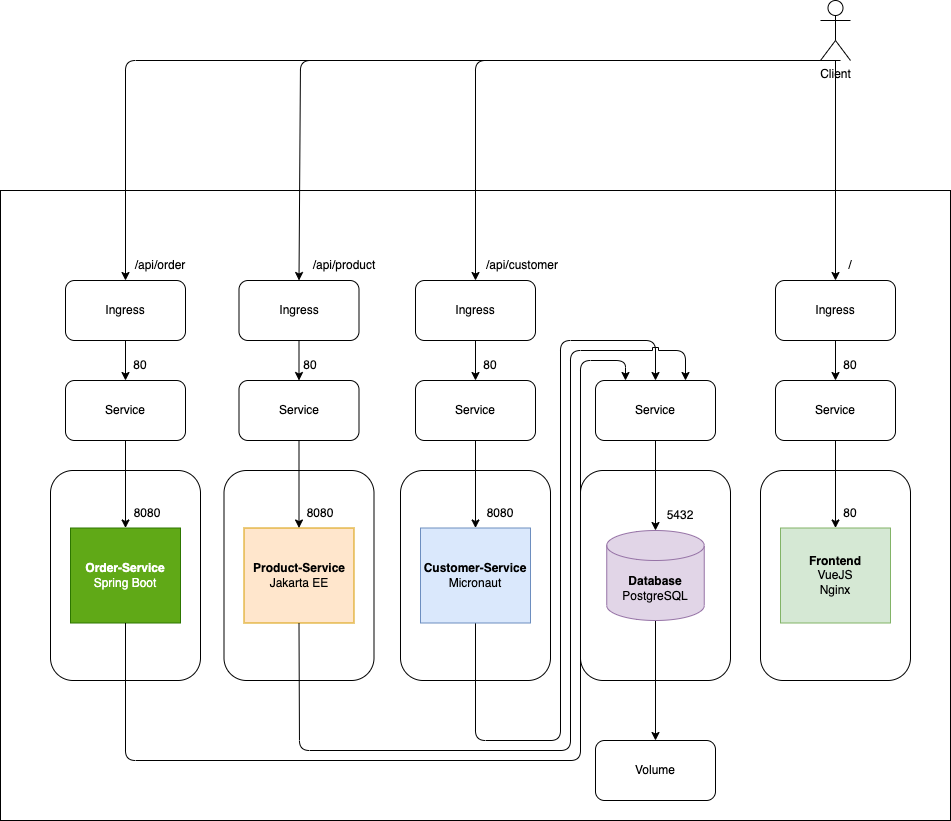
\includegraphics[width=1.0\textwidth]{../images/verteilungssicht/k8s-architektur.png}
    \caption{Aufbau der Infrastruktur auf Kubernetes}
    \label{fig:infrastruktur-k8s}
\end{figure}